% Created 2024-05-17 Fri 03:54
% Intended LaTeX compiler: lualatex
\documentclass[bigger]{beamer}
\usepackage{amsmath}
\usepackage{fontspec}
\usepackage{graphicx}
\usepackage{longtable}
\usepackage{wrapfig}
\usepackage{rotating}
\usepackage[normalem]{ulem}
\usepackage{capt-of}
\usepackage{hyperref}
\usetheme[progressbar=foot, sectionpage=none, numbering=fraction]{metropolis}
\usepackage{tikz}
\usepackage{booktabs}
\usepackage{adjustbox}
\usepackage{diagbox}
\usepackage{latexcolors}
\usetikzlibrary{automata, positioning, arrows, arrows.meta}
\usepackage{diagbox}
\usepackage{dsfont}
\usepackage{amsmath}
\usepackage{fontawesome}
\usepackage{pgfgantt}
\usepackage[ruled]{algorithm2e}
\usepackage[absolute, overlay]{textpos}
\definecolor{RedBrown}{RGB}{192, 4, 4} \setbeamercolor{progress bar}{fg=RedBrown} \setbeamercolor{title separator}{fg=RedBrown}
\setbeamercolor{progress bar in head/foot}{fg=RedBrown} \setbeamercolor{progress bar in section page}{fg=RedBrown} \setbeamercolor{alerted text}{fg=RedBrown}
\pretocmd{\tableofcontents}{\thispagestyle{empty}}{}{}
\addtocounter{framenumber}{-1}
\usepackage{listings}
\usepackage{xcolor}
\definecolor{codegreen}{rgb}{0,0.6,0}
\definecolor{codegray}{rgb}{0.5,0.5,0.5}
\definecolor{codepurple}{rgb}{0.58,0,0.82}
\definecolor{backcolour}{HTML}{f0f0f0}
\lstdefinestyle{mystyle}{
backgroundcolor=\color{backcolour},
commentstyle=\color{codegreen},
keywordstyle=\color{magenta},
numberstyle=\tiny\color{codegray},
stringstyle=\color{codepurple},
basicstyle=\ttfamily,
breakatwhitespace=false,
breaklines=true,
captionpos=b,
keepspaces=true,
numbers=none,
numbersep=5pt,
showspaces=false,
showstringspaces=false,
showtabs=false,
tabsize=2
}
\lstset{style=mystyle}
\usetheme{default}
\author{Andrea Pierré}
\date{May 17, 2024}
\title{Research plan}
\subtitle{Fleischmann -- Nassar joint meeting}
\institute{Brown University}
\titlegraphic{\hfill
\includegraphics[height=1.5cm]{img/Brown Logo_2016_2 Color Process ST_1300.png}}
\setbeamercovered{transparent=10}
\setbeamertemplate{section in toc}[sections numbered]
\AtBeginSection[]{\begin{frame}[plain, noframenumbering]{Outline}    \setbeamertemplate{section in toc}[sections numbered]\setbeamertemplate{subsection in toc}[subsections numbered]\vspace{-0.8em}\tableofcontents[currentsection, currentsubsection]\end{frame}}
\AtBeginSubsection[]{\begin{frame}[plain, noframenumbering]{Outline}\setbeamertemplate{section in toc}[sections numbered]\setbeamertemplate{subsection in toc}[subsections numbered]\tableofcontents[currentsection,currentsubsection]\end{frame}}
\hypersetup{
 pdfauthor={Andrea Pierré},
 pdftitle={Research plan},
 pdfkeywords={},
 pdfsubject={},
 pdfcreator={Emacs 29.3 (Org mode 9.7)}, 
 pdflang={English}}
\begin{document}

\maketitle
\begin{frame}[plain]{Outline}
\tableofcontents
\end{frame}

\section{Conceptual directions \& questions \faicon{question-circle}}
\label{sec:orga5c26cb}
\begin{frame}[<+->][label={sec:org422f1d5}]{What do we want to know?}
\begin{itemize}
\item Understand what the network learns
\(\to\) What \alert{function} does it learns?
\item How the constrains of the task affect learning \& the representations learned?
\item Does the network learn something related to the real neurons? (million \faicon{dollar}\faicon{dollar}\faicon{dollar} question)
\end{itemize}
\end{frame}
\begin{frame}[label={sec:orgf3fe8b7}]{Compositional hypothesis}
\begin{itemize}
\item From indexed locations (current) to coordinate system \(\to\) does the network learn a generalizable policy?
\item Merged actions space
\end{itemize}
\end{frame}
\begin{frame}[label={sec:orgdb095a5}]{Compositional hypothesis}
\begin{center}
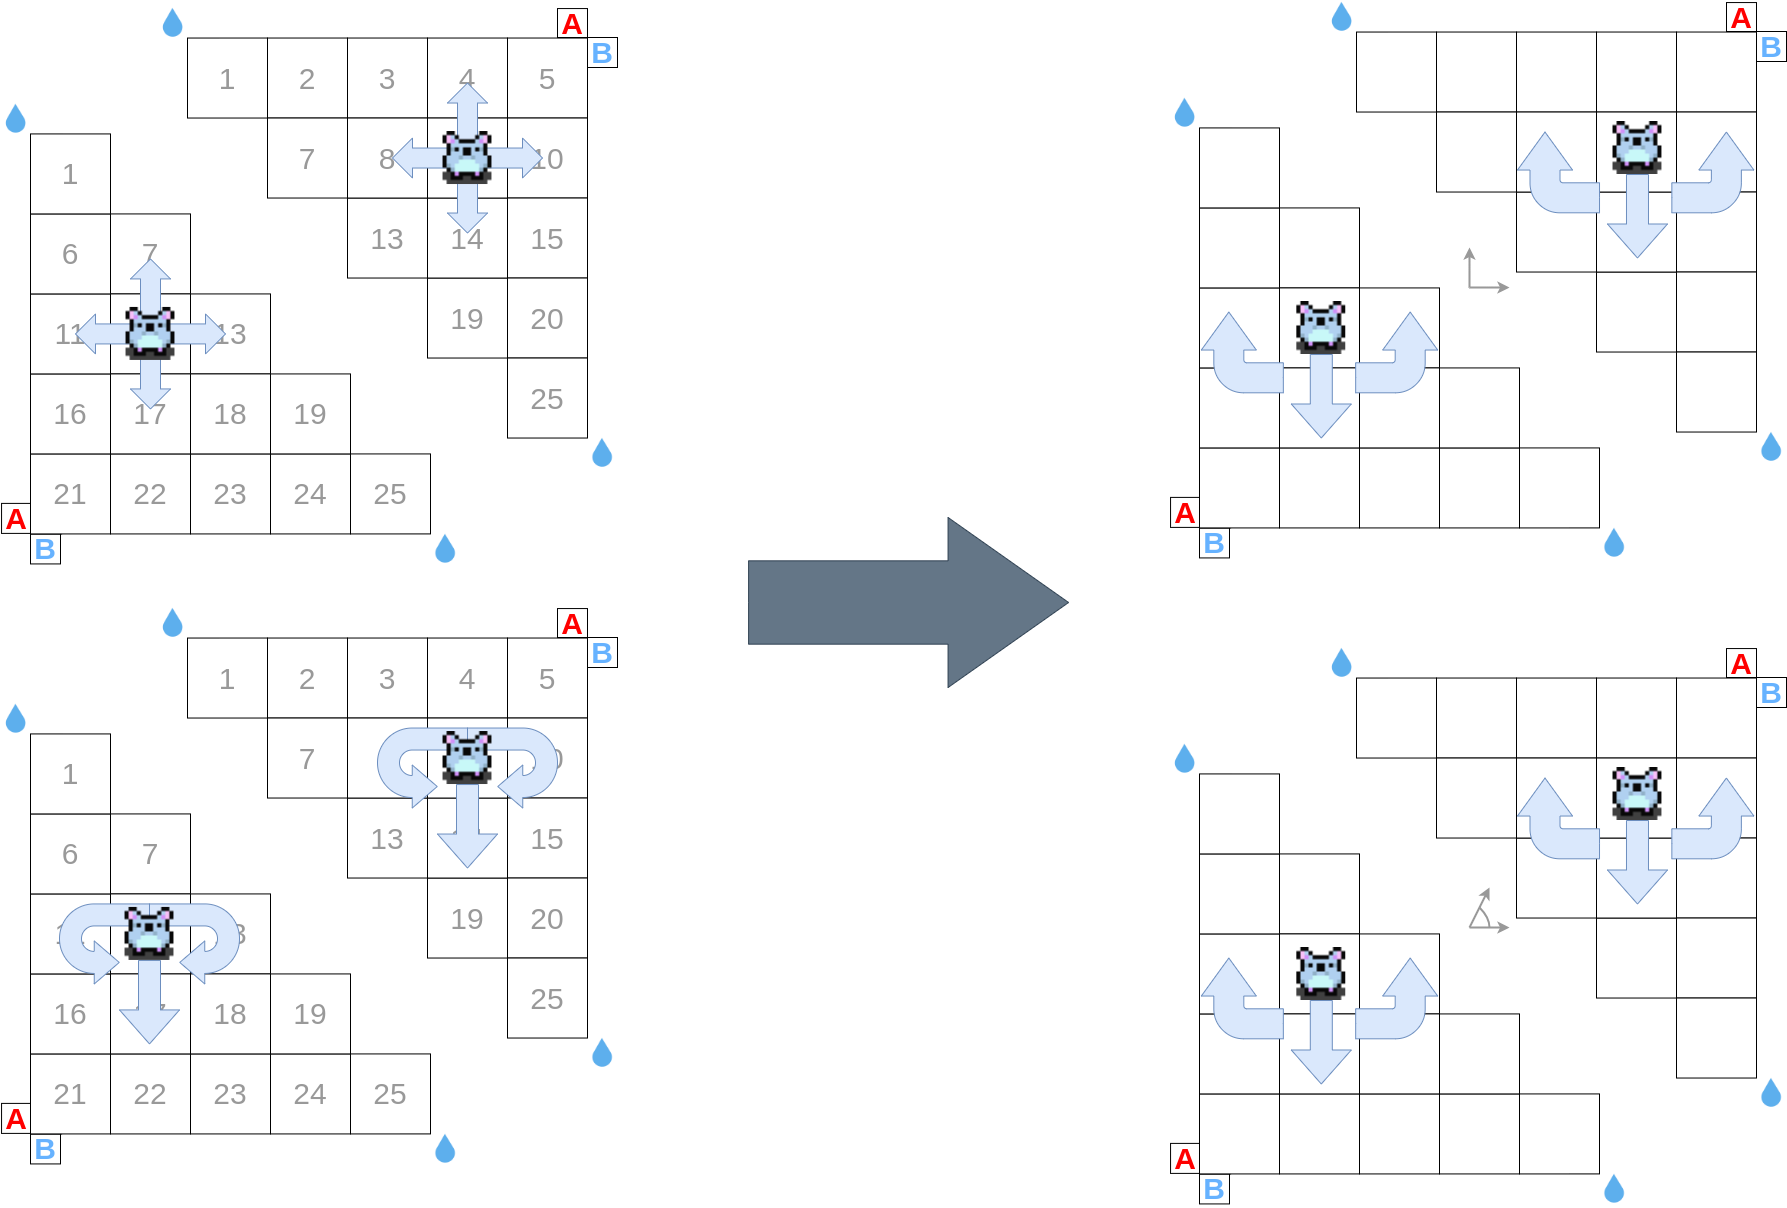
\includegraphics[width=.9\linewidth]{img/env_new-triangle-task.drawio.png}
\end{center}
\end{frame}
\begin{frame}[label={sec:org5cd5afd}]{Implementation}
\begin{center}
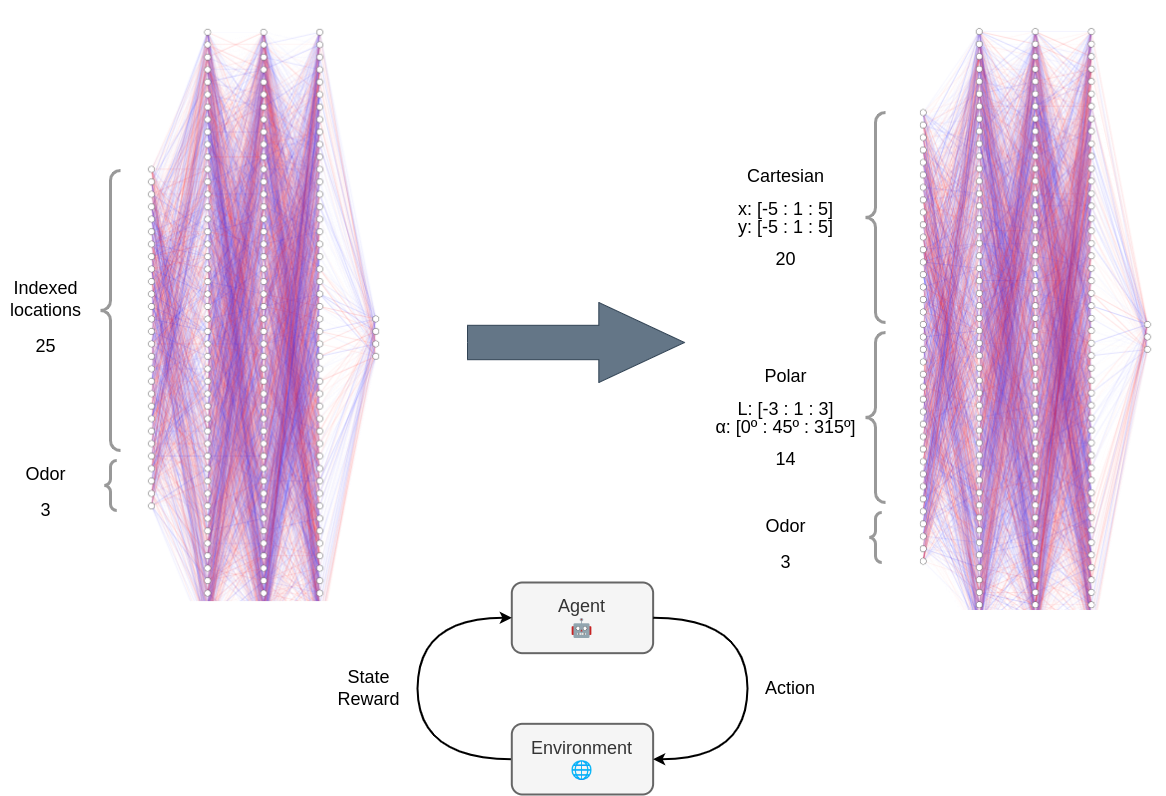
\includegraphics[width=.9\linewidth]{img/nn.drawio.png}
\end{center}
\end{frame}
\section{Experiments \& expected results \faicon{eyedropper} \faicon{area-chart}}
\label{sec:orgca6f00f}
\begin{frame}[<+->][label={sec:org772cab1}]{1) How training impacts the representations learned?}
\begin{itemize}
\item Feed both coordinates information (Cartesian \& polar) to the input layer (+ merge actions spaces in a common one)
\item Train on left/right task \(\to\) we expect the weights are close to zero on Cartesian representation?
\item Train on east/west task \(\to\) we expect the weights are close to zero on polar representation?
\item Not clear to me how to extract/define which neurons belong/contribute to Cartesian/polar representation
\end{itemize}
\end{frame}
\begin{frame}[label={sec:orga34032d}]{1) How training impacts the representations learned?}
\begin{center}
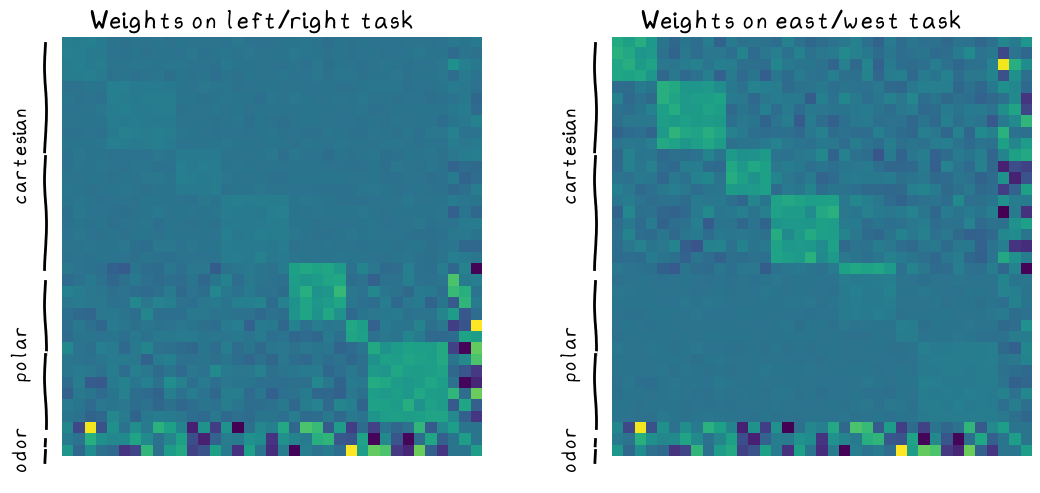
\includegraphics[width=.9\linewidth]{img/exp1-weights-heatmap.png}
\end{center}
\end{frame}
\begin{frame}[<+->][label={sec:org8e0c19d}]{2) Does the network learn a coordinate system?}
\begin{enumerate}
\item After training, move the population of agents in a translated coordinate system
\(\to\) we expect the population of agents to be able to solve the task with zero shot learning
\item Train with both coordinates information (Cartesian \& polar), after training feed incorrect polar angles
\begin{itemize}
\item On the left/right task \(\to\) we expect the population of agents still solves the task consistently
\item On the east/west task \(\to\) we expect the network doesn't converge to a stable policy (i.e all the agents don't solve the task consistently)
\end{itemize}
\end{enumerate}
\end{frame}
\begin{frame}[label={sec:org3ecf81b}]{2) Does the network learn a coordinate system?}
\begin{center}
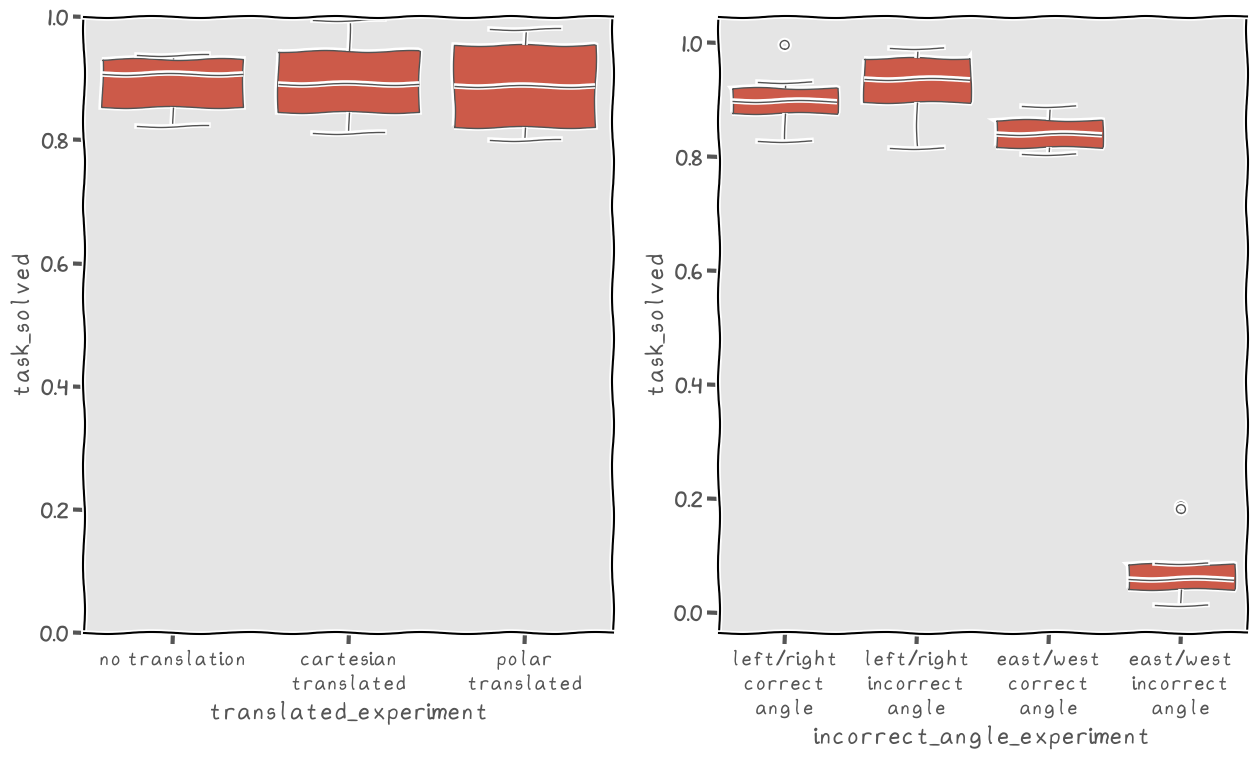
\includegraphics[width=.9\linewidth]{img/exp2-boxplot.png}
\end{center}
\end{frame}
\begin{frame}[<+->][label={sec:orgd1b69a9}]{3) Conjunctive odor-place coding}
\begin{itemize}
\item Train a population of agents, then after training, flip odor A and odor B in the task
\item In general we expect to find a population of conjunctive neurons that get active with the combination of both odor and specific location
\item Do the conjunctive cells get conserved or remapped? (Not clear to me, I'd expect they get remapped)
\end{itemize}
\end{frame}
\section{Roadmap \faicon{road}}
\label{sec:org61e243e}
\begin{frame}[<+->][label={sec:orgacec153}]{Milestones/how to get there}
\begin{enumerate}
\item Rewrite the environment(s) \faicon{star}\faicon{star}\faicon{star-o}
\begin{enumerate}
\item Code logic for new environment \colorbox{black!15!white}{[$\textasciitilde$1 week]}
\item Check everything works as expected (unit testing) \colorbox{black!15!white}{[$\textasciitilde$1 week]}
\item Bugs? \colorbox{black!15!white}{[$\textasciitilde$1 week]}
\end{enumerate}
\item Baseline training on new environment (convergence, hyperparameter tweaking, etc.) \faicon{star}\faicon{star}\faicon{star}\faicon{warning} \colorbox{black!15!white}{[1 week -- 1 month]}
\item Experiments
\begin{enumerate}
\item Task code \faicon{star}\faicon{star-o}\faicon{star-o} \colorbox{black!15!white}{[$\textasciitilde$1 week]}
\item Training \faicon{star}\faicon{star}\faicon{star-o}\faicon{warning} \colorbox{black!15!white}{[$\textasciitilde$2 week]}
\item Analysis code \faicon{star}\faicon{star}\faicon{star-o} \colorbox{black!15!white}{[$\textasciitilde$2 week]}
\end{enumerate}
\end{enumerate}
\end{frame}
\begin{frame}[label={sec:orged85e83},standout]{~}
Thanks!
\end{frame}
\end{document}
